% Generated by verification/make_review_draft.py
% Submission source SHA256: f845780cb4e91b0f1b2964da75be4b2b5c756327da7a37df377a7e6d4a2f6546
\documentclass[final,5p,times,twocolumn]{elsarticle}
\usepackage[T1]{fontenc}
\usepackage{microtype}
\usepackage{amsmath,amssymb,amsthm,mathtools,enumitem,booktabs}
\usepackage{graphicx,tikz}
\usepackage{float}
\floatstyle{plain}
\newfloat{algorithm}{tbp}{loa}
\floatname{algorithm}{Algorithm}
\usepackage{pgfplots}
\pgfplotsset{compat=1.18}
\usetikzlibrary{arrows.meta,positioning,shapes.geometric}
\definecolor{cellblue}{RGB}{40,95,150}
\definecolor{cellorange}{RGB}{190,100,25}
\usepackage[hidelinks]{hyperref}
\setlength{\emergencystretch}{3em}
\newtheorem{theorem}{Theorem}[section]
\newtheorem{lemma}[theorem]{Lemma}
\newtheorem{proposition}[theorem]{Proposition}
\newtheorem{corollary}[theorem]{Corollary}
\theoremstyle{definition}\newtheorem{definition}{Definition}[section]
\theoremstyle{remark}\newtheorem{remark}[theorem]{Remark}
\newcommand{\R}{\mathbb R}\newcommand{\Q}{\mathbb Q}\newcommand{\Z}{\mathbb Z}
\newcommand{\eps}{\varepsilon}
\newcommand{\poly}{\operatorname{poly}}
\newcommand{\osc}{\operatorname{osc}}
\newcommand{\bits}{\operatorname{bits}}
\newcommand{\norm}[1]{\lVert#1\rVert}
\journal{Operations Research Letters}

\newcommand{\reviewnote}[3]{\par\medskip\noindent
\begingroup\setlength{\fboxsep}{6pt}\fcolorbox{#1}{#1!5}{%
\begin{minipage}{\dimexpr\linewidth-2\fboxsep-2\fboxrule\relax}
\small\textbf{#2}\par\smallskip #3
\end{minipage}}\endgroup\par\medskip}
\newcommand{\leanchecked}[1]{\reviewnote{cellblue}{LEAN CHECKED --- conditional}{#1}}
\newcommand{\humancheck}[1]{\reviewnote{cellorange}{HUMAN REVIEW}{#1}}

\begin{document}
\begin{frontmatter}
\title{A short proof of a range-relative FPTAS for polynomial integer optimization over bounded polyhedra}
\author{Robert Hildebrand}
\ead{rhil@vt.edu}
\affiliation{organization={Grado Department of Industrial and Systems Engineering, Virginia Tech},
  city={Blacksburg}, state={Virginia}, country={USA}}
\begin{abstract}
We give a short proof of a fully polynomial-time range-relative approximation scheme for polynomial optimization over the integer points of a bounded rational polyhedron in fixed dimension. Boundedness supplies a finite slack decomposition and a finite integer objective range. The proof combines the reflecting-set decomposition of Cook, Hartmann, Kannan, and McDiarmid with Markov's polynomial derivative inequality and uses one integer linear feasibility query per refined cell. The running time is polynomial in the input encoding size, the numerical degree, and the reciprocal accuracy.
\end{abstract}
\begin{keyword}
Integer programming \sep Polynomial optimization \sep Approximation schemes \sep Fixed dimension \sep Reflecting cells
\end{keyword}
\end{frontmatter}
\reviewnote{cellblue}{ANNOTATED REVIEW COPY --- not the submission version}{
Blue notes identify specific Lean conclusions under explicit hypotheses; they do not certify entire surrounding statements. Amber notes identify remaining proof obligations and attribution checks. All 118 declarations are covered by the axiom audit. Classical Markov estimates are assumptions, not proved here. The paper's finite decomposition, algorithm and running time are not fully formalized.}
\humancheck{Suggested reading order: (1) Lemma~\ref{lem:arrangement} and the cost accounting; (2) the integral-slice scaling and barycentric geometry and remaining complexity accounting; (3) the passage from the actual cells to the conditional Lean theorem; (4) the two Markov hypotheses; (5) the comparisons and citations. Check these arguments independently rather than treating a successful Lean run as evidence for them.}


\section{Introduction and main result}

Let $P=\{\mathbf{x}\in\R^d:A\mathbf{x}\le\mathbf b\}$ be a bounded rational polyhedron, with $A\in\Q^{m\times d}$ and $\mathbf b\in\Q^m$, and let $f\in\Z[x_1,\ldots,x_d]$. We study
\begin{equation}\label{eq:problem}
 \begin{aligned}
 \min\quad & f(\mathbf{x})\\
 \text{s.t.}\quad & A\mathbf{x}\le\mathbf b,\\
 & \mathbf{x}\in\Z^d.
 \end{aligned}
\end{equation}
When $P\cap\Z^d\ne\varnothing$, choose minimizers and maximizers $\mathbf{x}_{\min},\mathbf{x}_{\max}$ and write $f_{\min}=f(\mathbf{x}_{\min})$ and $f_{\max}=f(\mathbf{x}_{\max})$.

De Loera, Hemmecke, K\"oppe, and Weismantel established an FPTAS for nonnegative polynomial maximization and a range-relative scheme for arbitrary polynomials in fixed dimension~\cite{DHKW06,DHKW08}. We give a short geometric proof for the bounded integer problem, using integer linear feasibility and an explicit bit-complexity bound. The guarantee is invariant under translation of the objective; it is not a multiplicative approximation to a nonnegative minimum.

For continuous convex bodies, Piazzon and Vianello~\cite[Propositions~1--2]{PV} obtain range-relative approximation from polynomial norming meshes, selecting an arbitrary feasible representative in each sufficiently small box and applying Markov's inequality. Our refined reflecting cells provide feasible integer progressions, allowing error to be measured against the integer objective range rather than the continuous range.

The key ingredient is decomposition by relative constraint slacks. The reflecting sets of Cook, Hartmann, Kannan, and McDiarmid~\cite{CHKM} underpin their integer-hull analysis; related symmetric covers appear in the quadratic and cubic algorithms of Ari and Hildebrand~\cite{AHIQP,AH}, and dyadic slack grouping also appears in Wei's quadratic algorithm~\cite[Section~4.1]{Wei}. Here refinement produces long feasible integer progressions. Markov's polynomial derivative inequality~\cite[Theorem~5.1.8]{BorweinErdelyi} on these progressions controls the error at an integer optimum, allowing any feasible representative of its cell. The same representatives work for all polynomials of a prescribed degree.

Markov's inequality is essential to the polynomial cell bound: it controls variation relative to the integer objective range, so the required refinement depends only on degree and accuracy. A coefficient-based Lipschitz estimate alone could require refinement exponential in the input encoding size. The Lipschitz-based grid reduction of~\cite{DHKW08} can tolerate a large denominator because its integer solver depends polynomially on the denominator's bit length; explicit cell enumeration requires polynomially many cells.

\begin{figure*}[t]
\centering
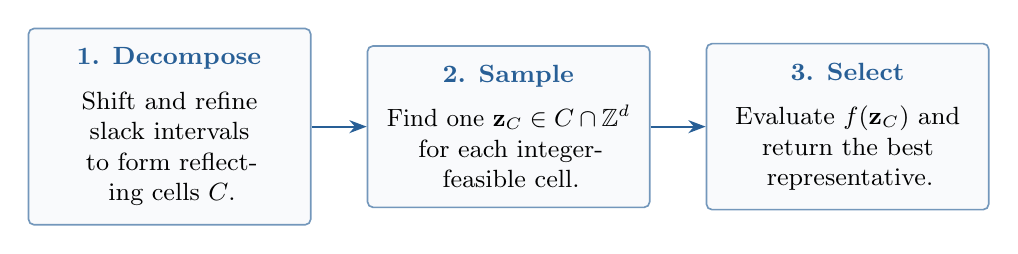
\begin{tikzpicture}[
  stage/.style={draw=cellblue!65,line width=.6pt,rounded corners=2pt,
    fill=cellblue!3,text width=.255\textwidth,minimum height=2.05cm,
    inner sep=7pt,align=center,font=\small},
  flow/.style={-{Stealth[length=2.2mm]},line width=.8pt,cellblue},
  node distance=7mm]
\node[stage] (decompose) {
  {\color{cellblue}\bfseries 1. Decompose}\\[5pt]
  Shift and refine slack intervals\\
  to form reflecting cells $C$.
};
\node[stage,right=of decompose] (sample) {
  {\color{cellblue}\bfseries 2. Sample}\\[5pt]
  Find one $\mathbf z_C\in C\cap\Z^d$\\
  for each integer-feasible cell.
};
\node[stage,right=of sample] (select) {
  {\color{cellblue}\bfseries 3. Select}\\[5pt]
  Evaluate $f(\mathbf z_C)$ and\\
  return the best representative.
};
\draw[flow] (decompose)--(sample);
\draw[flow] (sample)--(select);
\end{tikzpicture}
\caption{Algorithm at a glance: decompose a relaxation with the same integer points, select one representative from each cell containing integer points, and return the representative with the best objective value.}\label{fig:overview}
\end{figure*}

The algorithm follows the decompose--sample--select procedure summarized in Figure~\ref{fig:overview}. No local objective model is optimized. The proof separates the reflecting geometry (Section~\ref{sec:cover}) from enumeration and bit complexity (Section~\ref{sec:algorithm}).

To state the complexity bound precisely, we fix the following encoding convention. Vectors are columns and are written in bold. For an integer $u$, its \emph{binary encoding size} is $\langle u\rangle=1+\lceil\log_2(1+|u|)\rceil$, counting a sign bit and the binary magnitude bits. We use \emph{encoding size}, \emph{bit length}, or simply \emph{size} for storage measured in bits when the context is clear; \emph{magnitude} refers to the numerical absolute value. A rational number $u/v$ is stored in lowest terms with $v>0$, with size $\langle u/v\rangle=\langle u\rangle+\langle v\rangle$. For matrices, vectors, and lists, $\langle\cdot\rangle$ is the sum of the entry sizes together with the binary encoding sizes of the dimensions and list lengths. The polynomial is supplied explicitly as
\[
 f(\mathbf{x})=\sum_{\boldsymbol{\alpha}\in\mathcal A}c_{\boldsymbol{\alpha}}\mathbf{x}^{\boldsymbol{\alpha}},
 \qquad c_{\boldsymbol{\alpha}}\in\Z,\quad \boldsymbol{\alpha}\in\Z_+^d,\quad |\boldsymbol{\alpha}|_1\le D.
\]
Following~\cite{DHKW08}, coefficients are encoded in binary and exponent vectors in unary: each exponent $\alpha_j$ is stored as $\alpha_j$ one-bits followed by a zero, using $\alpha_j+1$ bits. The input is therefore a bit string, although exponents use unary rather than positional binary notation. Accordingly, $\langle f\rangle$ includes the coefficient sizes and $\sum_{\boldsymbol{\alpha}\in\mathcal A}\sum_{j=1}^d(\alpha_j+1)$, together with dimensions and list lengths. Write $\varphi=\langle A,\mathbf b,f,\eps\rangle$ for the total input encoding size. We set $D=\max\{1,\deg f\}$ from the nonzero monomials, taking $D=1$ for the zero polynomial; no separate degree input is needed. We retain $D$ explicitly in the running-time bound to show its contribution.

\begin{definition}[Range-relative FPTAS]\label{def:fptas}
Under the encoding convention above and for fixed dimension $d$, a range-relative fully polynomial-time approximation scheme is an algorithm that, for every rational $0<\eps\le1$, reports infeasibility when $P\cap\Z^d=\varnothing$, and otherwise returns $\mathbf{x}_{\eps}\in P\cap\Z^d$ satisfying
\begin{equation}\label{eq:guarantee}
 0\le f(\mathbf{x}_{\eps})-f_{\min}\le\eps(f_{\max}-f_{\min}).
\end{equation}
Its running time is polynomial in the total input encoding size $\varphi$ and $1/\eps$. The polynomial may depend on the fixed dimension. This is the fully polynomial-time weak-approximation notion of~\cite{DHKW08}. The maximization definition uses $f_{\max}-f(\mathbf{x}_{\eps})$ on the left.
\end{definition}

All complexity statements below count bit operations. The function $\poly$ denotes a polynomial with an absolute exponent, independent of $d,D,\eps$; different occurrences may denote different polynomials. Logs are base two unless indicated otherwise.

\humancheck{The final error is checked by \texttt{shifted\_slack\_cover\_guarantee}: actual integer rows, closed shifted-slack widths, and integrality imply progression samples in the original polytope. Coverage, complete feasible candidates, extrema and Markov remain inputs. Chamber construction, enumeration, and runtime remain unverified.}
\begin{theorem}[Polynomial approximation by reflecting cells]\label{thm:main}
Let $d\ge1$ and let $P=\{\mathbf{x}\in\R^d:A\mathbf{x}\le\mathbf b\}$ be bounded, with $A\in\Z^{m\times d}$ and $\mathbf b\in\Z^m$, let $f\in\Z[x_1,\ldots,x_d]$, and put $D=\max\{1,\deg f\}$, with $D=1$ when $f\equiv0$. For rational $0<\eps\le1$, let $\varphi=\langle A,\mathbf b,f,\eps\rangle$ be the total input encoding size.
There is a deterministic algorithm that reports infeasibility or returns $\mathbf{x}_{\eps}\in P\cap\Z^d$ satisfying~\eqref{eq:guarantee}, in at most
\begin{equation}\label{eq:runtime-coarse}
 \left(\frac{\varphi D}{\eps}\right)^{O(d)}
\end{equation}
bit operations, with an absolute constant in the $O(d)$ exponent.
\end{theorem}

Since the input explicitly lists the $m$ inequalities in $d$ variables, $m,d\le\varphi$; their separate factors in the detailed running-time bound are therefore absorbed into the base $\varphi$ and the $O(d)$ exponent in~\eqref{eq:runtime-coarse}. The dependence on dimension remains explicit in that exponent. More precisely, for fixed $P,D,d$, the algorithm makes $O(\eps^{-d/2})$ integer-feasibility queries; the detailed running-time bound in the proof retains the factor $\max\{D^2,D/\sqrt\eps\}$.

Rational inequalities can be normalized to integral data in polynomial time, as detailed below. Rational objective coefficients can likewise be reduced to integer coefficients by clearing denominators in polynomial time; positive scaling preserves the approximation guarantee, as in~\cite[Section~5]{DHKW08}. The remaining construction parameters and the exact feasibility-query count are introduced in the proof. For fixed $d$, the bound is polynomial in $\varphi$ and $1/\eps$, hence gives an FPTAS in Definition~\ref{def:fptas}. The same explicit bound remains valid for binary-encoded exponents, but then its numerical dependence on $D$ does not assert an FPTAS in the sparse binary input size.

The following guarantees were established by De Loera et al.~\cite[Theorem~1.1]{DHKW06}\cite[Theorems~1(a) and~2(b)]{DHKW08}; we include them to explain how our integer algorithm fits their approximation framework. The first is the elementary conversion from range-relative error to nonnegative maximization. The second follows their integral-slice scaling, barycentric rounding, and reduction to integer optimization~\cite[Section~3]{DHKW08}. We modify the rounding estimate using Markov's inequality to obtain a coefficient-independent grid multiplier, and substitute Theorem~\ref{thm:main} for their integer subroutine.

\leanchecked{\texttt{nonnegative\_maximization} proves the scalar conversion from range-relative error to a multiplicative bound when the minimum is nonnegative. Check that the maximization instance satisfies its hypotheses.}
\begin{corollary}[Nonnegative maximization {\cite[Theorem~1.1]{DHKW06}}]\label{cor:max}
Under the same assumptions and encoding conventions, if $f\ge0$ on $P\cap\Z^d$, choosing the largest objective value among the representatives yields
\[
 f(\mathbf{x}_{\eps})\ge(1-\eps)f_{\max}.
\]
Thus the construction gives a multiplicative FPTAS for nonnegative maximization under the encoding convention of Definition~\ref{def:fptas}.
\end{corollary}

\leanchecked{The new checks verify actual upward ceiling rounding, residual convex weights, the coordinatewise segment and grid identities, the ceiling multiplier, and the two-part error budget. The interval Markov inequality remains an explicit hypothesis. Integral-slice scaling, Carath\'eodory representation, the geometric assembly remain human-review obligations. The determinant/lcm encoding and runtime-exponent calculations are now checked conditional on stated preprocessing, encoding and solver bounds. Polynomial scaling and the scaled feasible-set bijection are checked separately.}
\begin{corollary}[Mixed-integer approximation {\cite[Theorems~1(a) and~2(b)]{DHKW08}}]\label{cor:mixed}
Fix the total dimension $d=d_c+d_i$. Let $P=\{\mathbf{x}\in\R^d:A\mathbf{x}\le\mathbf b\}$ be a bounded rational polyhedron and $f\in\Z[x_1,\ldots,x_d]$. Under the same encoding convention, for rational $0<\eps\le1$ there is an algorithm, polynomial in $\varphi=\langle A,\mathbf b,f,\eps\rangle$ and $1/\eps$, that reports infeasibility or returns
\[
\begin{gathered}\mathbf{x}_{\eps}\in P\cap(\Q^{d_c}\times\Z^{d_i}),\\
 0\le f(\mathbf{x}_{\eps})-f_{\min}\le\eps(f_{\max}-f_{\min}),
\end{gathered}\]
where the extrema are over $P\cap(\R^{d_c}\times\Z^{d_i})$. For nonnegative $f$ on this set, a multiplicative FPTAS for maximization is obtained as well. The running time is at most
\begin{equation}\label{eq:mixed-runtime}
 \left(\frac{\varphi D}{\eps}\right)^{O(d(d_c+1))}
\end{equation}
bit operations, with an absolute constant in the exponent.
\end{corollary}

\paragraph{Comparison with prior algorithms.}

The short rational generating functions used by De Loera et al. build on Barvinok's lattice-point counting algorithm~\cite{Barvinok}. Their approach~\cite{DHKW06,DHKW08} computes weighted sums involving $f^q$, where $q=O(1+\eps^{-1}\log N)$ and $N=|P\cap\Z^d|$. The standard Barvinok counting bound is $\langle A,\mathbf b\rangle^{O(d\log(d+1))}$~\cite[Theorem~2.3]{PakPanova}; our entire algorithm has bound $\varphi^{O(d)}$ for fixed $D,\eps$. This compares available upper bounds, not a runtime separation: counting alone does not describe their FPTAS, and our potentially large cell count does not establish practical superiority.

Del Pia's quadratic scheme~\cite[Proposition~3 and Section~6.2]{DelPia} uses affine optimization over boxes after geometric preprocessing, with flatness recursion in the remaining cases. For fixed quadratic rank $k$ and integer dimension $p$, it uses $O_{k,p}(1+\eps^{-k/2})$ MILP subproblems and allows variable continuous dimension. Our feasibility-call exponent matches $k/2$ at $k=d$, but our enumeration costs an additional factor of order $\eps^{-1/2}$. Our advantages are arbitrary degree and objective-independent representatives; we do not recover his low-rank dependence.

\section{Reflecting cells and approximation}\label{sec:cover}

We first construct cells supporting feasible integer progressions, then apply Markov's inequality along a progression through an integer optimum. Neither the optimum nor the objective range is needed by the algorithm.

\leanchecked{Rational row normalization: \texttt{commonDen\_pos} and \texttt{clearedEntry\_real} construct positive product denominators and integer coefficients, including the right-hand side. \texttt{cleared\_domain\_iff} preserves feasibility under any domain restriction. \texttt{cleared\_payload\_quadratic} bounds a row's integer payload by $L(L+2)$ for rational payload $L$; \texttt{cleared\_matrix\_payload} sums these bounds. The arithmetic operation cost remains unverified.}
Clear rational row denominators by multiplying each row by the product of its positive denominators. This takes polynomial time; normalized entries have $O(\varphi)$ bits. Equalities may be represented by pairs of inequalities, and lower-dimensional polytopes are allowed. Real feasibility and boundedness are testable by rational linear programming; boundedness remains a hypothesis of our theorem. After testing real feasibility, remove zero constraint rows. We treat $d\ge1$ below; dimension zero is immediate.

For the remainder of the construction, $A,\mathbf b$ denote the normalized integral data; $\varphi$ continues to denote the original input size. To track the construction explicitly, define
\begin{equation}\label{eq:tau}
 \tau=\left\lceil\log_2\bigl(2+\max\{\|A\|_{\max},\|\mathbf b\|_\infty\}\bigr)\right\rceil.
\end{equation}
In Schrijver's encoding convention~\cite[Section~2.1]{Schrijver}, each normalized row inequality has size at most $(d+1)(\tau+3)$, including its right-hand side. This bounds the per-inequality size parameter used by CHKM, distinct from our total input size $\varphi$. Here $\|A\|_{\max}$ is the largest absolute matrix entry, so $\tau$ bounds the coefficient bit lengths up to a constant. The remaining parameters have the following roles: $\Phi$ gives the common magnitude bound $2^\Phi$ for coordinates and shifted slacks and determines how many intervals $[2^k,2^{k+1}]$ are needed below, $\ell$ is the refinement, and $H$ bounds the number of hyperplanes. Set
\begin{align}
 \Phi&=5d^2(d+1)(\tau+3)+2,\label{eq:Phi}\\
 \ell&=\max\{D^2,\lceil D/\sqrt\eps\rceil\},\qquad H=m((\Phi+2)\ell+1),\label{eq:HT}\\
 R_d(H)&=\sum_{j=0}^{d}\binom Hj\le(1+H)^d.\label{eq:F}
\end{align}

Following the outward perturbation in~\cite[proof of Theorem~2.1, p.~29]{CHKM}, define
\[
\begin{gathered}
 \widetilde P=\{\mathbf{x}:A\mathbf{x}\le\mathbf b+\tfrac12\mathbf1\},\\
 s_i(\mathbf{x})=b_i+\tfrac12-\mathbf a_i^\top\mathbf{x}.
\end{gathered}
\]
\leanchecked{\texttt{integer\_row\_value}, \texttt{integer\_half\_shift}, and \texttt{shifted\_feasible\_iff} verify preservation of the integer feasible set for actual integer coefficient matrices. \texttt{shifted\_slack\_positive} proves the lower bound $1/2$. This shift is not a valid direct replacement for mixed-integer or continuous constraints.}
Since $A,\mathbf b$ are integral, $\widetilde P\cap\Z^d=P\cap\Z^d$. Every integer point of $P$ has $s_i\ge1/2$. We will extrapolate real segments in $\widetilde P$ and use integrality to return their integer samples to $P$. This shift is applied only to the pure-integer problem, including the scaled integer problem in the mixed-integer reduction.

\humancheck{External bound: CHKM, proof of Theorem~2.1, p.~29. Check the translation from their maximum inequality size to $(d+1)(\tau+3)$, the doubled shifted rows, extension from integer-hull vertices to integer points, and the separate $d=1$ case. The short version uses $\Phi=5d^2(d+1)(\tau+3)+2$. Lean's determinant estimates concern the different, sharper exponent retained in the long version; they do not formalize this imported bound.}
The coordinate and slack estimates in the proof of CHKM's Theorem~2.1~\cite[p.~29]{CHKM}, with their per-inequality size bounded by $(d+1)(\tau+3)$, give
\begin{equation}\label{eq:integer-bounds}
 |x_j|<2^\Phi,\qquad \tfrac12\le s_i(\mathbf{x})<2^\Phi
 \quad(\mathbf{x}\in P\cap\Z^d).
\end{equation}
Their estimates are stated at vertices of the integer hull and extend throughout that hull by linearity. Their integral shifted rows $2A\mathbf{x}\le2\mathbf b+\mathbf1$ have slacks $2s_i$; the extra constant in~\eqref{eq:Phi} safely covers this convention. Their argument treats $d\ge2$; for $d=1$, the same bounds follow directly from the interval endpoints and $|a_{ij}|,|b_i|<2^\tau$. Only bounds on integer feasible points are needed here. The extended version retains the detailed determinant proof with a sharper exponent.

We use the reflecting-set construction of CHKM~\cite[proof of Theorem~2.1, pp.~29--30]{CHKM}: move integer points into the interior and group slacks in dyadic intervals. Our modification subdivides each such interval into $\ell$ equal parts. This extends their reflection calculation to long integer progressions; see also~\cite[Theorem~2.2]{AH}. Figure~\ref{fig:pentagon-cells} illustrates the refinement.

\humancheck{Check that every original integer point lies strictly inside $Q$, that closures of full-dimensional chambers cover $Q$ when it has interior, and that empty interior implies integer infeasibility. Overlap at subdivision hyperplanes is intentional. Lean verifies the shifted feasible-set equality and the lower slack bound; it does not construct $Q$ or the chamber cover.}
\begin{definition}[Closed refined cells]\label{def:thresholds}
For integers $\Phi,\ell\ge1$, let
\begin{equation}\label{eq:thresholds}
\begin{split}
\mathcal B_{\Phi,\ell}=\{2^\Phi\}\cup\\
 \left\{2^k\left(1+\frac j\ell\right):-2\le k<\Phi,\ 0\le j<\ell\right\}.
\end{split}
\end{equation}
There are $(\Phi+2)\ell+1$ thresholds, starting at $1/4$. Set
\[
 Q=\{\mathbf{x}:1/4\le s_i(\mathbf{x})\le2^\Phi\ (1\le i\le m)\}.
\]
Subdivide $Q$ by the hyperplanes $s_i(\mathbf{x})=a$, $a\in\mathcal B_{\Phi,\ell}$. The family $\mathcal C$ consists of the closures of the resulting full-dimensional chambers. If $Q$ has empty interior, set $\mathcal C=\varnothing$.
\end{definition}

Every integer point of $P$ lies in the interior of $Q$, by~\eqref{eq:integer-bounds}, and therefore belongs to a closed cell. The cells may overlap on subdivision hyperplanes, but no separate lower-dimensional faces are needed. Conversely, $Q\subseteq\widetilde P$, so every integer point in a cell belongs to $P$. These statements also justify declaring integer infeasibility when $Q$ has empty interior. The set $Q$ is bounded: its recession directions satisfy $A\mathbf v=0$, which forces $\mathbf v=0$ since $P$ is nonempty and bounded.

If $a<b$ are successive thresholds, then
\begin{equation}\label{eq:width}
 b-a\le a/\ell.
\end{equation}
Indeed, on $[2^k,2^{k+1}]$ the spacing is $2^k/\ell$ and $a\ge2^k$. The same argument applies to the two additional scales below one.

\begin{figure*}[t]
\centering
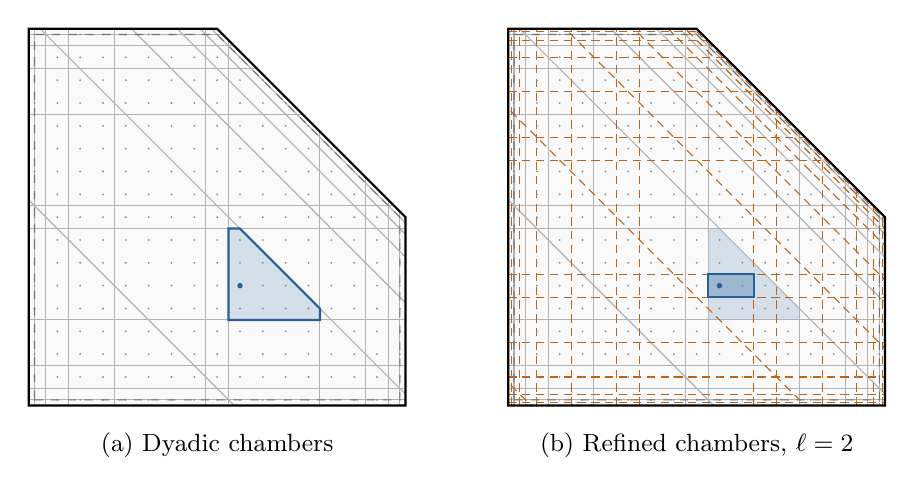
\begin{tikzpicture}[x=.29cm,y=.29cm,font=\small]
\foreach \shift/\panel/\refined in {0/{(a) Dyadic chambers}/0,21/{(b) Refined chambers, $\ell=2$}/1} {
 \begin{scope}[xshift=\shift*.29cm]
  \begin{scope}
   \clip (-.25,-.25)--(16.25,-.25)--(16.25,8)--(8,16.25)--(-.25,16.25)--cycle;
   \fill[gray!5] (-.25,-.25) rectangle (16.25,16.25);
   \fill[cellblue!20] (8.5,3.5)--(12.5,3.5)--(12.5,4)--(9,7.5)--(8.5,7.5)--cycle;
   \foreach \a in {.25,.5,1,2,4,8,16,32} {
    \draw[gray!60,thin] ({\a-.5},-.25)--({\a-.5},16.25);
    \draw[gray!60,thin] ({16.5-\a},-.25)--({16.5-\a},16.25);
    \draw[gray!60,thin] (-.25,{\a-.5})--(16.25,{\a-.5});
    \draw[gray!60,thin] (-.25,{16.5-\a})--(16.25,{16.5-\a});
    \draw[gray!60,thin] (-10,{34.5-\a})--(35,{-10.5-\a});
   }
   \ifnum\refined=1
    \foreach \a in {.375,.75,1.5,3,6,12,24} {
     \draw[cellorange,densely dashed,thin] ({\a-.5},-.25)--({\a-.5},16.25);
     \draw[cellorange,densely dashed,thin] ({16.5-\a},-.25)--({16.5-\a},16.25);
     \draw[cellorange,densely dashed,thin] (-.25,{\a-.5})--(16.25,{\a-.5});
     \draw[cellorange,densely dashed,thin] (-.25,{16.5-\a})--(16.25,{16.5-\a});
     \draw[cellorange,densely dashed,thin] (-10,{34.5-\a})--(35,{-10.5-\a});
    }
    \fill[cellblue!45] (8.5,4.5) rectangle (10.5,5.5);
    \draw[cellblue,thick] (8.5,4.5) rectangle (10.5,5.5);
   \else
    \draw[cellblue,thick] (8.5,3.5)--(12.5,3.5)--(12.5,4)--(9,7.5)--(8.5,7.5)--cycle;
   \fi
   \foreach \x in {0,...,16} {\foreach \y in {0,...,16} {
    \pgfmathtruncatemacro{\inside}{\x+\y<=24}
    \ifnum\inside=1 \fill[black!45] (\x,\y) circle (.045);\fi
   }}
  \end{scope}
  \draw[black!55,dashed] (0,0)--(16,0)--(16,8)--(8,16)--(0,16)--cycle;
  \draw[thick] (-.25,-.25)--(16.25,-.25)--(16.25,8)--(8,16.25)--(-.25,16.25)--cycle;
  \fill[cellblue] (9,5) circle (.12);
  \node[below] at (8,-1) {\panel};
 \end{scope}
}
\end{tikzpicture}
\caption{Closed shifted-slack chambers for $P=\{\mathbf{x}\in[0,16]^2:x_1+x_2\le24\}$ (dashed outline). The solid outline is $Q$, whose lower shifted-slack bound is $1/4$; the upper bound is inactive in this example. The fifth shifted slack is $24.5-x_1-x_2$, giving the diagonal lines. The shaded dyadic chamber is refined in (b); its darker closed rectangle $[8.5,10.5]\times[4.5,5.5]$ contains the representative $(9,5)$. All lattice points of $P$, including its boundary points, lie inside $Q$. Adjacent closed cells share their boundaries.}
\label{fig:pentagon-cells}
\end{figure*}

\leanchecked{\texttt{integer\_row\_value} and \texttt{integer\_half\_shift} imply \texttt{shifted\_feasible\_iff}. \texttt{shifted\_slack\_integral\_progression} then derives feasible integer samples in the original polytope from weak shifted-slack interval bounds. \texttt{shifted\_slack\_cover\_guarantee} connects them to the final error. Check that actual closed chambers satisfy the interval hypotheses and cover the integer feasible set. Real extrapolated points need only lie in $\widetilde P$.}
\begin{lemma}[Refined CHKM reflection property]\label{lem:reflection}
Each $C\in\mathcal C$ is described by $a_i\le s_i(\mathbf{x})\le c_i$ for successive thresholds $a_i<c_i$. Set
\[
 D_C=\{\mathbf v\in\R^d:|\mathbf a_i^\top\mathbf v|\le a_i\ (1\le i\le m)\}.
\]
Then $\ell(C-C)\subseteq D_C$ and $C\pm D_C\subseteq\widetilde P$. In particular,
\begin{equation}\label{eq:long}
 \mathbf{x}+k(\mathbf{y}-\mathbf{x})\in P\cap\Z^d
 \quad(\mathbf{x},\mathbf y\in C\cap\Z^d,\ k\in\Z,\ |k|\le\ell).
\end{equation}
\end{lemma}
\begin{proof}
The CHKM reflection calculation~\cite[p.~30]{CHKM} applies with the refined width:
\[
 |s_i(\mathbf y)-s_i(\mathbf{x})|\le c_i-a_i\le a_i/\ell
 \le s_i(\mathbf{x})/\ell.
\]
This gives both inclusions and the real progression in $\widetilde P$. Its integer samples belong to $P$ because the shift preserves integer feasibility. Boundedness of $D_C$ follows from $A\mathbf v=0\Rightarrow\mathbf v=0$.
\end{proof}

\humancheck{The full if-and-only-if characterization is not checked in Lean. Verify both endpoint implications, zero-slack rows, and the strict versus weak inequalities.}
\begin{remark}[Relative slacks characterize extrapolation]\label{rem:slack-characterization}
Let $\mathbf{x},\mathbf y\in\widetilde P$, set $\mathbf v=\mathbf y-\mathbf{x}$, and let $\ell>0$. The segments $\mathbf{x}+[-\ell,\ell]\mathbf v$ and $\mathbf y+[-\ell,\ell]\mathbf v$, centered at $\mathbf{x}$ and $\mathbf y$ respectively, both lie in $\widetilde P$ if and only if, for every row $i$,
\[
 \ell\,|s_i(\mathbf y)-s_i(\mathbf{x})|
 \le\min\{s_i(\mathbf{x}),s_i(\mathbf y)\}.
\]
Indeed, the minimum slack along the first segment is $s_i(\mathbf{x})-\ell|s_i(\mathbf y)-s_i(\mathbf{x})|$, and similarly for the second. For positive slacks the condition is equivalently
\[
 \frac{\max\{s_i(\mathbf{x}),s_i(\mathbf y)\}}
 {\min\{s_i(\mathbf{x}),s_i(\mathbf y)\}}\le1+\frac1\ell;
\]
if either slack is zero, both must be zero. Our cells have positive shifted slacks, so this last case never arises. Thus multiplicative slack control is exactly the geometry needed for extrapolation about both points. Refined dyadic intervals enforce this condition with short rational descriptions, and integrality limits the number of relevant scales. The condition is independent of the objective: Proposition~\ref{prop:extrema} turns the resulting cover into a simultaneous approximation guarantee for every polynomial of degree at most $D$.
\end{remark}

The integer progression property is the geometric input to approximation. Closed chambers also give weak linear descriptions directly; integer rounding below only removes threshold denominators.

\humancheck{Check the chamber count $\sum_{j=0}^d\binom Hj$, its recurrence, and the two closed-halfspace enumeration with nonempty-interior tests. Zero normals must be removed first. Check compression to $2m$ bounds and rounding $[a,c]$ to $[\lceil a-1/2\rceil,\lfloor c-1/2\rfloor]$ for the original integer slack. Enumeration, rounding encoding bounds and runtime are not formalized.}
\begin{lemma}[Number, encoding, and enumeration of cells]\label{lem:arrangement}
The closed cells can be enumerated deterministically in $(\varphi\ell)^{O(d)}$ bit operations, and their number is at most $(\varphi\ell)^{O(d)}$. Each cell has a description by at most $2m$ weak linear inequalities of total encoding size $\poly(\varphi)$. Rounding its slack bounds gives a closed rational subset $\widehat C$ with exactly the same integer points, described by at most $2m$ inequalities whose coefficient bit lengths are $O(\tau+\Phi+1)$, independent of $\ell$.
\end{lemma}
\begin{proof}
With $H=m((\Phi+2)\ell+1)$, the standard arrangement bound gives $R_d(H)$ chambers~\cite{Stanley}; intersecting with convex $Q$ cannot increase their number. The thresholds have denominator dividing $4\ell$ and numerator bit length $O(\Phi+\log(\ell+1))$.

Incrementally split each closed cell into its two closed halfspace intersections, retaining only those with nonempty interior. These cover the parent, including the splitting hyperplane. At most $R_d(H)$ cells occur at each stage. Their constraints compress to two bounds per original row. Interior is tested by maximizing $\delta\in[0,1]$ with a common margin $\delta$ in every inequality; positivity is equivalent to nonempty interior since zero normals were removed. Thus $O((H+1)R_d(H))$ rational LP tests suffice. Since $m,d,\tau=O(\varphi)$, $\Phi=O(d^3(\tau+1))$, and $\log(\ell+1)=O(\log(D+1)+\langle\eps\rangle)$, each test has polynomial encoding size and the total enumeration cost is $(\varphi\ell)^{O(d)}$.

Finally, replace $a\le s_i(\mathbf{x})\le c$ by
\[
 \lceil a-\tfrac12\rceil\le b_i-\mathbf a_i^\top\mathbf{x}
 \le\lfloor c-\tfrac12\rfloor.
\]
This preserves integer points, defines a subset of the closed cell, and removes the dependence on $\ell$ from the coefficient bit lengths. The extended version gives the enumeration details.
\end{proof}

\begin{remark}[Parallel families]
If row $i$ contributes $q_i$ distinct threshold hyperplanes, the count can be sharpened to
\[
 |\mathcal C|\le
 \sum_{\substack{I\subseteq\{1,\ldots,m\}\\|I|\le d}}
 \prod_{i\in I}q_i
 \le\sum_{j=0}^d\binom mj((\Phi+2)\ell+1)^j.
\]
The insertion argument counts intersections involving at most one hyperplane from each parallel family; further dependencies can only reduce the count. This improves the bound without changing its worst-case $\ell^d$ dependence. We retain $R_d(H)$ for simplicity. The boundary-vertex count in~\cite[pp.~30--31]{CHKM} bounds integer-hull vertices, not all reflecting cells, and therefore does not directly replace this count.
\end{remark}

We next combine the sample-to-supremum argument used in polynomial norming meshes~\cite[proof of Proposition~2]{PV} with a second-difference bound at a discrete minimum. Long progressions control variation between integer samples without assuming continuous stationarity.

We use the classical Markov inequality~\cite[Theorem~5.1.8]{BorweinErdelyi}, rescaled to an interval: every real polynomial $q$ of degree at most $D$ satisfies
\[
 \|q'\|_{\infty,[u,v]}\le\frac{2D^2}{v-u}\|q\|_{\infty,[u,v]},\qquad u<v.
\]

\leanchecked{\texttt{sampled\_markov} proves the displayed bound. The even-part identity and degree contraction are proved by \texttt{even\_contract} and \texttt{degree\_contract}; \texttt{symmetrized\_difference} proves the sharper half-degree constant. Only the centered and interval classical Markov derivative estimates are explicit external hypotheses. Check their scaling and degree parameters against Pierzchala Theorem~1.1.}
\begin{lemma}[Approximation at a discrete minimum]\label{lem:markov}
Let $D\ge1$ and $\ell\ge D^2$ be integers, and let $p\in\R[t]$ have degree at most $D$. Suppose
\[
 a\le p(k)\le b\quad(k=-\ell,\ldots,\ell),\qquad p(-1)\ge p(0).
\]
Then
\[
 p(1)-p(0)\le \frac{D^2}{\ell^2}(b-a).
\]
\end{lemma}
\begin{proof}
Set $q=p-(a+b)/2$ and $W=\|q\|_{\infty,[-\ell,\ell]}$. The scaled classical Markov inequality gives $\|q'\|_\infty\le D^2W/\ell$; see~\cite[Theorem~5.1.8]{BorweinErdelyi}. Every point of $[-\ell,\ell]$ lies within $1/2$ of a sampled integer, so
\[
 W\le \frac{b-a}{2}+\frac{D^2}{2\ell}W\le\frac{b-a+W}{2},
 \qquad W\le b-a.
\]
Let $n=\lfloor D/2\rfloor$. The even part of $q$ has the form
\[
 e(t)=\frac{q(t)+q(-t)}2=h(t^2),\qquad \deg h\le n.
\]
Thus $\|h\|_{\infty,[0,\ell^2]}\le W$. Markov's inequality on $[0,\ell^2]$ gives $\|h'\|_\infty\le 2n^2W/\ell^2$. Since $\ell\ge1$, the mean value bound on $[0,1]$ and $p(-1)\ge p(0)$ yield
\[
\begin{aligned}
 p(1)-p(0)&\le p(1)+p(-1)-2p(0)\\
 &=2(h(1)-h(0))\\
 &\le\frac{4\lfloor D/2\rfloor^2}{\ell^2}(b-a)
 \le\frac{D^2}{\ell^2}(b-a).
\end{aligned}
\]
For $D=1$, $h$ is constant and the bound is zero. The argument also covers $a=b$.
\end{proof}

The estimate is needed only on the cell containing a global minimizer, and holds for any representative of that cell. Applying it also to $-f$ gives the following simultaneous approximation of both extrema. The general conversion from a polynomial norming inequality to range-relative optimization is given in~\cite[Proposition~1]{PV}; here we use the discrete-minimum estimate directly. The reflecting geometry supplies the feasible integer samples needed here.

\leanchecked{\texttt{eval\_restrict} and \texttt{degree\_restrict} construct the genuine multivariate line restriction. \texttt{multivariate\_selection} proves feasible minimum selection given a reflecting witness; the shifted slack-cover theorem derives its progression witness from rowwise slack widths, coordinate integrality, coverage and oracle completeness. The maximum follows in the paper by negating $f$; check that translation separately.}
\begin{proposition}[Representatives approximate extrema]\label{prop:extrema}
Choose one integer representative from each integer-feasible closed cell, forming $Y$. If $P\cap\Z^d\ne\varnothing$ and $\ell\ge D^2$, then every real polynomial $f$ of degree at most $D$ satisfies
\[
\begin{aligned}
 0&\le\min_Y f-\min_{P\cap\Z^d} f\le\frac{D^2}{\ell^2}(f_{\max}-f_{\min}),\\
 0&\le\max_{P\cap\Z^d} f-\max_Y f\le\frac{D^2}{\ell^2}(f_{\max}-f_{\min}).
\end{aligned}
\]
\end{proposition}
\begin{proof}
Let $\mathbf{x}_{\min}$ minimize $f$ on $P\cap\Z^d$, and let $\mathbf{y}$ represent a cell containing it. Put $p(t)=f(\mathbf{x}_{\min}+t(\mathbf{y}-\mathbf{x}_{\min}))$. Lemma~\ref{lem:reflection} makes all integer samples with $|k|\le \ell$ feasible, so they lie between $f_{\min}$ and $f_{\max}$. Minimality gives $p(-1)\ge p(0)$. Lemma~\ref{lem:markov} now bounds $f(\mathbf{y})-f(\mathbf{x}_{\min})$. Apply the same argument to $-f$ for the maximum.
\end{proof}



\section{Algorithm and complexity}\label{sec:algorithm}

Algorithm~\ref{alg:sampling} enumerates the refined cells and compares their representatives. It accepts any degree bound $D\ge\max\{1,\deg f\}$; Theorem~\ref{thm:main} computes this bound from $f$. A constant objective requires only one integer feasibility query, and dimension zero is immediate. Representatives may be processed as a stream or saved for reuse.

\begin{algorithm}[tbp]
\centering
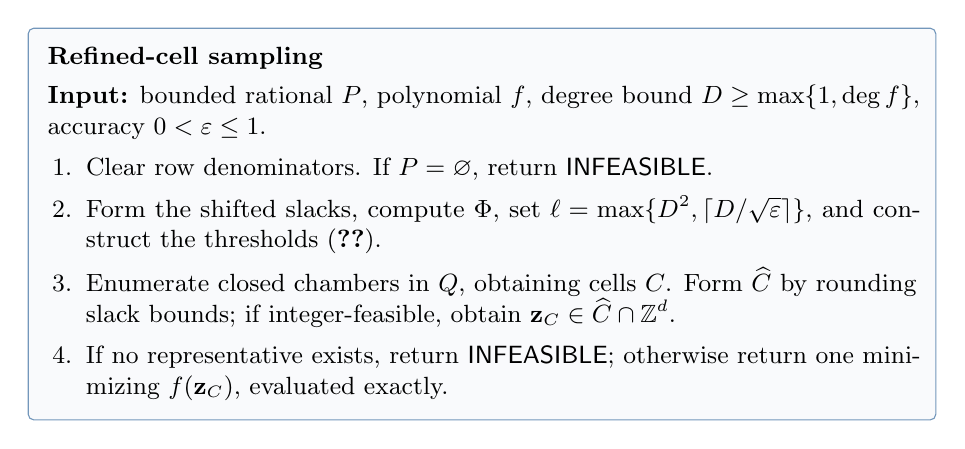
\begin{tikzpicture}
\node[draw=cellblue!65,rounded corners=2pt,fill=cellblue!3,inner sep=7pt] {
\begin{minipage}{.91\columnwidth}\small
\textbf{Refined-cell sampling}\par\smallskip
\textbf{Input:} bounded rational $P$, polynomial $f$, degree bound $D\ge\max\{1,\deg f\}$, accuracy $0<\eps\le1$.
\begin{enumerate}[leftmargin=1.5em,itemsep=2pt,topsep=4pt]
\item Clear row denominators. If $P=\varnothing$, return \textsf{INFEASIBLE}.
\item Form the shifted slacks, compute $\Phi$, set $\ell=\max\{D^2,\lceil D/\sqrt\eps\rceil\}$, and construct the thresholds~\eqref{eq:thresholds}.
\item Enumerate closed chambers in $Q$, obtaining cells $C$. Form $\widehat C$ by rounding slack bounds; if integer-feasible, obtain $\mathbf z_C\in\widehat C\cap\Z^d$.
\item If no representative exists, return \textsf{INFEASIBLE}; otherwise return one minimizing $f(\mathbf z_C)$, evaluated exactly.
\end{enumerate}
\end{minipage}};
\end{tikzpicture}
\caption{The cover and representatives depend only on $P,D,\eps$.}
\label{alg:sampling}
\end{algorithm}

\leanchecked{\texttt{ceiling\_refinement} proves positivity, $\ell\ge D^2$, and $D^2/\ell^2\le\eps$ for the actual maximum/ceiling choice. \texttt{slack\_cover\_guarantee} connects the rowwise geometry and integrality to the final error. \texttt{empty\_candidates\_iff} checks infeasibility conditional on sound and complete oracles.}
\begin{proof}[Correctness in Theorem~\ref{thm:main}]
Every integer-feasible cell contributes a feasible representative, and the closed cells cover $P\cap\Z^d$. Thus $Y=\varnothing$ if and only if $P\cap\Z^d=\varnothing$. Otherwise, Proposition~\ref{prop:extrema} and $\ell=\max\{D^2,\lceil D/\sqrt\eps\rceil\}$ give
\[
 0\le\min_Y f-f_{\min}\le \frac{D^2}{\ell^2}(f_{\max}-f_{\min})\le\eps (f_{\max}-f_{\min}).
\]
The algorithm returns a minimizer on $Y$. The cover and representatives depend only on $P,D,\eps$, so the same set works for every polynomial of degree at most $D$.
\end{proof}

\humancheck{The rest of this complexity argument is not Lean checked. Reconcile the LP test count with the integer-oracle call count; verify Kannan's bound, objective evaluation cost, rational arithmetic and the absorption into $\varphi^{O(d)}$. An abstract existence theorem for a best candidate does not certify this algorithmic cost.}
It remains to account for bit operations. There are three costs: constructing the arrangement, producing integer representatives, and evaluating the objective. The distinction between the number of cells and the sizes of their descriptions is important: refinement increases the former polynomially in $1/\sqrt\eps$, whereas it increases the threshold bit lengths only logarithmically.
Lemma~\ref{lem:arrangement} bounds the chamber enumeration cost. The bit length of $\ell$ is $O(\log(D+1)+\langle\eps\rangle)$; compute the least positive integer $k$ satisfying $\eps k^2\ge D^2$ by binary search with rational comparisons, and set $\ell=\max\{D^2,k\}$. Generating all thresholds uses $O(\Phi\ell)$ arithmetic operations on integers with $O(\Phi+\log(\ell+1))$ bits and is included in the arrangement bound when $m\ge1$. A nonempty bounded polyhedron in positive dimension cannot be specified by zero inequalities.

Once a cell has been enumerated, its integer feasibility query has a description whose coefficient sizes do not grow with the refinement parameter.
Each of at most $R_d(H)$ queries has $d$ integer variables and a total encoding size
\begin{equation}\label{eq:ilp-size}
 S_C=O\!\left(m(d+1)(\tau+\Phi+1)+d+m\right).
\end{equation}
Fixed-dimensional integer linear feasibility with witness production takes $2^{O(d\log(d+1))}S_C^{O(1)}$ bit operations using Kannan's algorithm~\cite{Kannan}, improving the dimension dependence of Lenstra's algorithm~\cite{Lenstra}. Every integer point returned from a shifted cell belongs to the original bounded polytope. Accordingly, every returned coordinate has at most $\Phi+O(1)$ bits by~\eqref{eq:integer-bounds}; its bit length grows logarithmically with its magnitude. Notice also that~\eqref{eq:ilp-size} has no dependence on $\ell$ other than the number of cells, because the threshold inequalities have already been rounded to integer slack bounds.

Finally, the coordinate bound ensures that exact objective evaluation also has polynomial bit cost, even though feasible coordinates can be numerically large.
The integer coefficients of $f$ have bit length at most $\langle f\rangle$. If $\mathbf{x}\in P\cap\Z^d$, every monomial has absolute value at most $2^{D\Phi}$. Each value of $f(\mathbf{x})$, and the intermediates obtained by evaluating monomials and summing them, has $O(\langle f\rangle+D\Phi+\log(|\mathcal A|+1))$ bits. Repeated squaring evaluates the explicit exponent vectors in a number of arithmetic operations polynomial in $\langle f\rangle+d+\log(D+1)$. Even schoolbook integer arithmetic therefore gives
\begin{equation}\label{eq:eval}
 \poly(\langle f\rangle+d+D\Phi)
\end{equation}
bit operations per representative. The case of the zero polynomial is immediate. Returning an exact integer objective value also fits this bound. No unit-cost assumption on rational arithmetic is used.

By Lemma~\ref{lem:arrangement}, the number of cells and enumeration steps is $(\varphi\ell)^{O(d)}$, since $m,d,\tau=O(\varphi)$ and $\Phi=O(d^3(\tau+1))$. Under our unary-exponent encoding, $D=O(\varphi)$ and all auxiliary bit lengths are polynomially bounded in $\varphi$. Each enumeration test and objective evaluation therefore has polynomial bit cost, and each integer-feasibility query takes $2^{O(d\log(d+1))}\poly(\varphi)$ bit operations. Substituting $\ell=\max\{D^2,\lceil D/\sqrt\eps\rceil\}$ gives the total running time $(\varphi D/\eps)^{O(d)}$, proving Theorem~\ref{thm:main}. For binary-encoded exponents, the per-query and evaluation bounds instead retain a factor $\poly(\varphi,D)$, which is also absorbed into this total bound.

For fixed $P,D,d$, the number of integer-feasibility queries is $O(\eps^{-d/2})$. Objective coefficients enter only through exact evaluation~\eqref{eq:eval}. Normalization preserves polynomial encoding size, so the bound also applies to rational inequalities.

\begin{proof}[Proof of Corollary~\ref{cor:max}]
Applying Proposition~\ref{prop:extrema} to $-f$ gives $f_{\max}-f(\mathbf{x}_{\eps})\le\eps (f_{\max}-f_{\min})$. Nonnegativity on $P\cap\Z^d$ implies $f_{\max}-f_{\min}\le f_{\max}$.
\end{proof}

\leanchecked{\texttt{rounded\_barycentric\_weights} and \texttt{rounded\_segment\_weights} check the actual ceiling-rounded weights and construct nonnegative residual weights summing to one. \texttt{barycentric\_coordinate\_segment} checks the segment identity. \texttt{rounded\_grid\_coordinate} provides an explicit integer numerator over $k\Delta$. \texttt{markov\_grid\_multiplier} and its bounds theorem check the ceiling choice and half-error budget. \texttt{unit\_interval\_markov\_error} derives the segment estimate from the classical derivative bound. \texttt{markov\_grid\_transfer} checks the final error composition; the older Lipschitz and range-gap helpers are no longer needed.}
\humancheck{Check DHKW Lemma 9, the Carath\'eodory representation and choice of largest weight, convex membership from the residual weights, and the assembly of the scalar and coordinatewise Lean results. The actual determinant size, lcm positivity/divisibility and length, and $Q$ length are checked by \texttt{integer\_basis\_determinant\_size}, \texttt{basis\_lcm\_spec}, \texttt{basis\_lcm\_size}, and \texttt{mixed\_grid\_size}. Polynomial size absorption and the final exponent are checked by \texttt{mixed\_grid\_polynomial\_size}, \texttt{mixed\_scaled\_input\_size}, \texttt{mixed\_runtime\_composition}, and \texttt{mixed\_runtime\_exponent}. Cost bounds for enumeration, lcm computation and the integer solver are inputs, not certified implementations. Check their instantiation and the remaining normalization and grid-multiplier encoding bounds. Positive polynomial scaling, integer coefficients, degree, feasible-set identification, and scaled encoding bounds remain checked in ScaledPolynomial.}
\begin{proof}[Proof of Corollary~\ref{cor:mixed}]
If $d_c=0$, apply Theorem~\ref{thm:main}. Otherwise set $r=d_c$ and $S=P\cap(\R^r\times\Z^{d_i})$. By~\cite[Lemma~9]{DHKW08}, an integer $\Delta>0$ of polynomial encoding size in fixed dimension can be computed such that every nonempty slice $\Delta P_{\mathbf z}$ is integral. We modify the barycentric rounding in~\cite[Lemma~10]{DHKW08} and use Markov's inequality instead of a coefficient-based Lipschitz estimate. Set
\[
 k=\left\lceil\frac{4D^2r(r+1)}{\eps}\right\rceil,
 \qquad Q=k\Delta,\qquad t=\frac{r(r+1)}k.
\]
For any $\mathbf x\in P_{\mathbf z}$, Carath\'eodory's theorem gives $\mathbf x=\sum_{i=0}^r\lambda_i\mathbf v_i$ for slice vertices $\mathbf v_i\in\Delta^{-1}\Z^r$ and convex weights, indexed so that $\lambda_0\ge1/(r+1)$. Put
\[
 \mu_i=\frac{\lceil k\lambda_i\rceil}{k}\ (i\ge1),
 \qquad \mu_0=1-\sum_{i=1}^r\mu_i.
\]
For $i\ge1$, $\lambda_i\le\mu_i\le\lambda_i+1/k$, while
$\mu_0\ge\lambda_0-r/k\ge(1-t)\lambda_0$. Since $0<t\le1$, all weights are nonnegative and $\mu_i\ge(1-t)\lambda_i$. Therefore
\[
 \mathbf y=\sum_{i=0}^r\mu_i\mathbf v_i
 =(1-t)\mathbf x+t\mathbf w\in P_{\mathbf z}\cap Q^{-1}\Z^r
\]
for some $\mathbf w\in P_{\mathbf z}$: its convex weights are $(\mu_i-(1-t)\lambda_i)/t$.

Write $R=f_{\max}-f_{\min}$ over $S$. The polynomial
$p(u)=f((1-u)\mathbf x+u\mathbf w,\mathbf z)-f_{\min}$ has degree at most $D$ and lies in $[0,R]$ on $[0,1]$. Markov's inequality gives
\[
 |f(\mathbf y,\mathbf z)-f(\mathbf x,\mathbf z)|
 \le2D^2tR\le\eps R/2.
\]
Thus the grid preserves nonemptiness and approximates the minimum within $\eps R/2$, including when $R=0$. Apply Theorem~\ref{thm:main} on the grid with accuracy $\eps/2$. Its objective range is at most $R$, so the total error is at most $\eps R$.

Substitute $\mathbf x=\mathbf u/Q$ and use the integer polynomial $g(\mathbf u,\mathbf z)=Q^D f(\mathbf u/Q,\mathbf z)$. Its degree and support are unchanged, and coefficient bit lengths increase by $O(D\log(Q+1))$. Since
\[
 \log Q=\log\Delta+
 O\!\left(\log(D+1)+\log(r+1)+\log(1/\eps)\right),
\]
positive scaling preserves the guarantee; negation and nonnegativity give the maximization claim. For explicit complexity, normalize the inequalities to integers and let $\tau$ bound their coefficient bit lengths. DHKW construct $\Delta$ as the least common multiple of nonzero absolute determinants of $r$-row bases of the continuous-variable matrix~\cite[proof of Lemma~9]{DHKW08}. Hadamard's inequality gives
\[
 \log\Delta=O\!\left(\binom mr r(\tau+\log(r+1))\right).
\]
Enumerating these bases and computing their least common multiple takes $\varphi^{O(r+1)}$ bit operations; normalization changes encoding size only polynomially. The scaled input has size at most $\varphi^{O(r+1)}$ under our unary-exponent convention. Applying Theorem~\ref{thm:main} proves~\eqref{eq:mixed-runtime}. For binary exponents, the extra polynomial dependence on $D$ is likewise absorbed into the displayed bound.

The new grid multiplier avoids the coefficient Lipschitz constant and positive range-gap bound in DHKW's reduction. This sharpens the sufficient grid resolution, but does not alone establish a better overall asymptotic runtime: the integer solvers depend on $\log Q$, and the common denominator $\Delta$ remains.
\end{proof}

\humancheck{The integer-hull vertex observation and proposed extensions are not formally checked. In particular, low rank and nonpolyhedral domains are directions, not consequences of the current FPTAS.}
\section{Discussion and extensions}\label{sec:conclusion}
For any refinement $\ell\ge1$, the representatives include every vertex of the integer hull. Indeed, if such a vertex $\mathbf v$ shared a cell with a distinct integer point $\mathbf y$, reflection would make $2\mathbf v-\mathbf y$ feasible, contradicting extremality of $\mathbf v=(\mathbf y+(2\mathbf v-\mathbf y))/2$. Thus every linear objective is optimized exactly.

The reflecting cover is independent of objective coefficients, so its representatives can be reused for any polynomial of degree at most $D$. Multiplicative slack bins connect the construction to approximate Pareto methods~\cite{PY} and affine slicing~\cite{HWZ}; Markov-based norming meshes provide the continuous sampling analogue~\cite[Propositions~1--3]{PV}. Our error certificate uses feasible integer samples and the integer objective range.

Cook, Hartmann, Kannan, and McDiarmid also give a fully polynomial-time approximation scheme for lattice-point counting in fixed dimension~\cite[Theorem~3.1]{CHKM}. Its dense-lattice case uses volume estimates, while its thin case recurses on lower-dimensional slices. Combining this architecture with Markov estimates suggests an alternative route to polynomial optimization, replacing volume estimates by feasible sampling. Establishing the range-relative guarantee and bit complexity would require further analysis; the refined reflecting cover gives the direct proof used here.

A simple principle allows other local procedures: if $|f-h_C|\le\delta_C$ on the feasible part of each cell and a feasible candidate minimizes $h_C$ there within $\eta_C$, selecting the best candidate has error at most $2\delta_{C^*}+\eta_{C^*}$, where $C^*$ contains a global optimum. Indeed, compare the candidate to that optimum through $h_{C^*}$ and apply the two residual bounds. An FPTAS also needs polynomial bounds on construction, local computation, and encoding.

For a supplied factorization $f(\mathbf{x})=g(B\mathbf{x})+\mathbf c^\top\mathbf{x}$ with few rows in $B$, affine optimization could handle the remaining directions without refinement. Obtaining a rank-sensitive cover with sufficient feasible samples is an open direction for this approach; changing the oracle alone does not reduce our cell count. Likewise, extension to a bounded nonpolyhedral set requires a cover supporting the same feasible progressions and tractable integer-feasibility queries. An outer polyhedral relaxation alone does not ensure that reflected points remain feasible.

For continuous extensions, Pierzcha\l a~\cite[Theorem~1.4]{Pierzchala} proves that polynomial images of compact Markov sets remain Markov sets when the map has full generic rank in the target. Combined with~\cite[Proposition~2]{PV}, this supplies norming meshes on further continuous sets. It does not supply integer representatives or uniform encoding bounds for the Markov constants, and hence does not by itself extend our integer FPTAS.

\section*{AI assistance and formal verification}
Robert Hildebrand posed the approximation question, proposed using the CHKM decomposition from the Ari--Hildebrand work, and directed the mathematical scope, encoding analysis, comparisons, and revisions. OpenAI's Codex assistant contributed mathematical exploration, proposed arguments, literature searches, drafting, and computational checks. The extended manuscript records these contributions in detail; responsibility for the manuscript remains with the human author.

The accompanying Lean development contains 118 checked results, including the even-part polynomial identity and degree bound, the strengthened $D^2/\ell^2$ sampled Markov estimate, affine line restriction, and representative selection. It also verifies $\ell=\max\{D^2,\lceil D/\sqrt\eps\rceil\}\ge D^2$ and $D^2/\ell^2\le\eps$. The classical Markov inequalities on $[-\ell,\ell]$ and $[0,\ell^2]$ are explicit hypotheses, not custom axioms. The shifted cover theorem verifies the half-unit relaxation for actual integer rows and derives samples feasible in the original polytope from closed shifted-slack widths and integrality. The mixed-integer checks verify upward-rounded barycentric weights, their residual convex weights and segment identity, the grid-coordinate identity, the ceiling multiplier, and the final error budget. The segment estimate assumes the classical Markov bound on $[0,1]$. Integral-slice scaling, Carath\'eodory representations and their geometric assembly remain external inputs. The scaled polynomial is constructed over the integers with its substitution identity, support and degree verified. The scaled feasible-set bijection and binary-length bounds for polynomial coefficients and scaled constraints are also verified. Rational row normalization preserves feasibility with verified bit-length bounds. The extended version's determinant and slack estimates are checked conditional on Cramer data and convex representations; the invocation of CKHM's integer-hull estimates here is not formalized. The determinant and least-common-multiple size bounds and mixed-integer runtime exponent calculation are also checked, conditional on polynomial encoding and subroutine cost bounds. Construction costs and full bit complexity remain unverified. Sources, checker scripts, and verification logs are maintained with the extended manuscript.

\humancheck{Reference audit: journal numbering for DHKW and Del Pia was checked against supplied published PDFs. The SODA page range has been completed. Piazzon--Vianello Propositions 1--3, Borwein--Erdelyi Theorem 5.1.8, and Pierzchala Theorems 1.1 and 1.4 were checked against the supplied full texts. Their continuous results do not certify the integer-range argument. Wei is retained as the user-supplied Optimization Online preprint; no arXiv record was located. The CHKM p.~29 locator was checked against the supplied published PDF. Still check the Stanley chapter DOI, PY metadata and Pak--Panova journal numbering. See \texttt{verification/reference\_audit.txt} for remaining source-access limitations.}
\begin{thebibliography}{99}
\bibitem{AH} C.~Ari and R.~Hildebrand.
\emph{Hidden Convexity via Symmetric Displacement Covers: Mixed-Integer Quadratic Programming and Integer Cubic Programming in Fixed Dimension}.
arXiv:2609.18266, version~2, September~23, 2026.
\url{https://arxiv.org/abs/2609.18266v2}.

\bibitem{AHIQP} C.~Ari and R.~Hildebrand.
\emph{Bounded Integer Quadratic Programming through Parallelepiped Covers and Discrete Convic Optimization}.
arXiv:2609.17889, 2026.
\url{https://arxiv.org/abs/2609.17889}.

\bibitem{Wei} L.~Wei.
\emph{Integer quadratic programming in fixed dimension is polynomial-time solvable}.
Optimization Online, 2026.
\url{https://optimization-online.org/wp-content/uploads/2026/09/integer-quadratic-programming-arxiv.pdf}.

\bibitem{Stanley} R.~P.~Stanley.
An introduction to hyperplane arrangements.
In \emph{Geometric Combinatorics}, IAS/Park City Mathematics Series, vol.~13,
American Mathematical Society, 2007, pp.~389--496.
\url{https://doi.org/10.1090/pcms/013/08}.

\bibitem{CHKM} W.~Cook, M.~Hartmann, R.~Kannan, and C.~McDiarmid.
On integer points in polyhedra.
\emph{Combinatorica} 12 (1992), 27--37.
\url{https://doi.org/10.1007/BF01191202}.

\bibitem{DHKW06} J.~A.~De~Loera, R.~Hemmecke, M.~K\"oppe, and R.~Weismantel.
Integer polynomial optimization in fixed dimension.
\emph{Mathematics of Operations Research} 31 (2006), 147--153.
\url{https://doi.org/10.1287/moor.1050.0169}.

\bibitem{DHKW08} J.~A.~De~Loera, R.~Hemmecke, M.~K\"oppe, and R.~Weismantel.
FPTAS for optimizing polynomials over the mixed-integer points of polytopes in fixed dimension.
\emph{Mathematical Programming} 115 (2008), 273--290.
\url{https://doi.org/10.1007/s10107-007-0175-8}.

\bibitem{PakPanova} I.~Pak and G.~Panova.
On the complexity of computing Kronecker coefficients.
\emph{Computational Complexity} 26 (2017), 1--36.
\url{https://doi.org/10.1007/s00037-015-0109-4}.

\bibitem{PY} C.~H.~Papadimitriou and M.~Yannakakis.
On the approximability of trade-offs and optimal access of Web sources.
\emph{Proceedings of the 41st Annual Symposium on Foundations of Computer Science}, 2000, 86--92.
\url{https://doi.org/10.1109/SFCS.2000.892068}.

\bibitem{HWZ} R.~Hildebrand, R.~Weismantel, and K.~Zemmer.
An FPTAS for minimizing indefinite quadratic forms over integers in polyhedra.
\emph{Proceedings of the 2016 Annual ACM--SIAM Symposium on Discrete Algorithms}, 2016, pp.~1715--1723.
\url{https://doi.org/10.1137/1.9781611974331.ch118}.

\bibitem{DelPia} A.~Del~Pia.
An approximation algorithm for indefinite mixed integer quadratic programming.
\emph{Mathematical Programming} 201 (2023), 263--293.
\url{https://doi.org/10.1007/s10107-022-01907-3}.

\bibitem{Lenstra} H.~W.~Lenstra, Jr.
Integer programming with a fixed number of variables.
\emph{Mathematics of Operations Research} 8 (1983), 538--548.
\url{https://doi.org/10.1287/moor.8.4.538}.

\bibitem{Kannan} R.~Kannan.
Minkowski's convex body theorem and integer programming.
\emph{Mathematics of Operations Research} 12 (1987), 415--440.
\url{https://doi.org/10.1287/moor.12.3.415}.

\bibitem{Schrijver} A.~Schrijver.
\emph{Theory of Linear and Integer Programming}. Wiley, Chichester, 1986.

\bibitem{BorweinErdelyi} P.~Borwein and T.~Erd\'elyi.
\emph{Polynomials and Polynomial Inequalities}. Graduate Texts in Mathematics 161, Springer, New York, 1995.
\url{https://doi.org/10.1007/978-1-4612-0793-1}.

\bibitem{Barvinok} A.~I.~Barvinok.
A polynomial time algorithm for counting integral points in polyhedra when the dimension is fixed.
\emph{Mathematics of Operations Research} 19 (1994), 769--779.
\url{https://doi.org/10.1287/moor.19.4.769}.

\bibitem{Pierzchala} R.~Pierzcha\l a. Markov's inequality and polynomial mappings.
\emph{Mathematische Annalen} 366 (2016), 57--82.
\url{https://doi.org/10.1007/s00208-015-1294-9}.

\bibitem{PV} F.~Piazzon and M.~Vianello.
Markov inequalities, Dubiner distance, norming meshes and polynomial optimization on convex bodies.
\emph{Optimization Letters} 13 (2019), 1325--1343.
\url{https://doi.org/10.1007/s11590-018-1377-0}.
\end{thebibliography}
\end{document}
